\documentclass{article}
\usepackage[utf8]{inputenc}

\title{COMP6703 \ Group \ Project}
\author{Ruosong\ Yang, \ Zhiyuan\  Wen}
\date{December 2018}


\usepackage{biblatex}
\addbibresource{ref.bib}
% \usepackage{natbib}
\usepackage{graphicx}
\usepackage{amsmath}
\usepackage[UTF8]{ctex}
\usepackage[top=2cm, bottom=2cm, left=2cm, right=2cm]{geometry}
\usepackage{algorithm}
\usepackage{algorithmicx}
\usepackage{algpseudocode}
\usepackage{url}
\usepackage{amssymb}
\begin{document}



\maketitle

\section{Problem introduction}
\noindent
For Flowers Recognition, it is an image classification problem. Classification means a discriminative model is needed to determine the types of given image. More specifically, in this problem, we need to classify each image into five classes: \textbf{chamomile, tulip, rose, sunflower, dandelion}. \\

\noindent
For the dataset, it contains \textbf{4242} images, and each image has about \textbf{340 * 280} pixels. For each class, there are nearly \textbf{800} images. \textbf{(这里,做表1(overview of each classes and total numbers), 图1 (插入一个图片例子))}\\
\noindent
The data comes from \textit{Flickr}, \textit{Google images}, and \textit{Yandex images}.
There are also many applications of image classification. The first application is a personal photo organization. Take \textit{Eden Photos}, a Mac OS application for photo organization, as an example. It uses \textit{Imagga’s} image recognition to offer its users' image tags, automatic keywording of photos, and auto-categorization based on visual topics. Users can sync their photos’ metadata on all devices and get keyword search in the native Photos app on their iPhones too. And a powerful commercial use of image recognition can be seen in the field of stock photography and video. Stock websites provide platforms where photographers and video-makers can sell their content. Contributors need a way to tag large amounts of visual material, which is time-consuming and tedious. In the same time, without proper keyword attribution, their content cannot be indexed – and thus cannot be discovered by buyers.


\section{Steps in the KDD(Knowledge Discovery in Databases) process}
\noindent
\textbf{Describe each step in the KDD process that you perform and explain your choice of transformation techniques and algorithms, etc.}\\

\noindent
The standard KDD process contains 5 steps: Selection, Prepossessing, Transformation, Data Mining, Interpretation/Evaluation \cite{fayyad1996data}.\\

\begin{figure}[h]
    \centering
    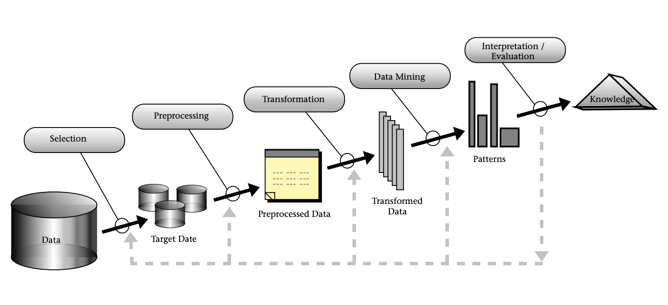
\includegraphics[scale=0.4]{kdd_process.png}
    \caption{An Overview of the Steps That Compose the KDD Process\cite{fayyad1996data}}
    \label{fig:kdd_process}
\end{figure}

\subsection{Step One}
\noindent
Step One consists of both data collection and selection. The goal of data collection is for target data for data mining to be first identified. Such data can be either internal or external. Internal
data refers to all kinds of data that are kept within an organization whereas external data refers to data that can be collected from external sources such as those relating to competitors or the social media, etc. The goal of data selection is concerned with the selection of a subset of data for data mining. By a subset of data, it can mean a subset of attributes/features/variables, or a subset of data/records sampled from internal or external data sources. Data selection is sometimes performed with the use of different methodologies or algorithms.

\noindent
In this step, we just collect our data from \cite{flower_dataset}, a overview of data is in \textbf{figure1}, then we split all data to train-validation as \textbf{8:2}, which means \textbf{80\%} of the data is training set, and \textbf{20\%} of the data is validation set, as shown in \textbf{Table2}.




\subsection{Step Two}
bla
\subsection{Step Three}
bla
\subsection{Step Four}
bla
\subsection{Step Five}
bla

\section{Algorithm selection}
\noindent
\textbf{Since there is a chance that you will have to try different ways of transforming data and different algorithm, you may like to explain the criteria for your considerations.}\\


\section{Fine tuning}
\noindent
\textbf{If there is a requirement for parameters of different algorithms to be tuned, explain how you arrive at particular values.}


\section{Assumptions and tricks}
\noindent
\textbf{Discuss any modeling assumptions as well as practical “hacks” you made in your model.}

\section{Performances and analyses}
\noindent
\textbf{Report the results of your tests and performance assessment of the models constructed. The results can be presented in terms of classification or prediction accuracy or root mean squared error (RMSEs). Investigation of parameter effects will be necessary.} \\

\noindent
\textbf{Try to interpret the results of your model and provide some theoretical justification why the algorithms of your choice should work.}

\section{Appendices}
Provide an appendix with the relevant portions of your code. Input-output
routines should not be included. Provide a list of any external tools that you have used. If you use an existing technique, for example decision tree, Support Vector Machine, EM-algorithm, LSA etc., provide an appendix that shortly (less than 1 page) describes that technique.\\

\noindent
You are required to include references. If you are using information or tools from other sources apart from your own you should reference them. Avoid copying pieces of text from books or papers. If you have to do it, paraphrase and reference it.


\printbibliography
\end{document}

